در این بخش به بنا کردن چهارچوب نظریه‌ای پرداخته می‌شود که نقش کلیدی در فهم شکل‌های غشا‌های غول‌آسا داشته است. این نظریه بر اساس انرژی الاستیک خمش غشا ایجاد شده‌است. همچنین در این نظریه حل‌شوندگی بسیار کم ملکول‌های لیپیدی و تاثیر اختلاف فشار اسمزی به شکل قید روی سطح و حجم غشا در نظر گرفته شده است. درواقع جذابیت این نظریه در توصیف تبادل بین انرژی‌هایی است با منشا موضعی و سراسری. از طرفی شکل انحنای غشا بر اساس انرژی‌های ناشی از خمش‌های موضعی (خمش میانگین و خمش گاووسی) تعیین می‌شود و از طرف دیگر با فرض اینکه غشا تغییر توپولوژیکی نداشته باشد (با غشای دیگری جوش نخورد، تکه‌ای از غشا به شکل جوانه از آن جدا نشود، یا حفره‌ای در آن ایجاد نشود) سطح و حجم ثابتی خواهد داشت که بر شکل نهایی که غشا می‌تواند به خود بگیرد تاثیر بسیار مشخصی دارد. ارتباط میان پدیده‌های موضعی و سراسری با دو کمیت به نام تنش مکانیکی
\LTRfootnote{mechanical tension}  
$\gamma_{ten}$
و اختلاف فشار
$\Delta P$
برقرار می‌شود.

نظریه‌ی مدل خمش ذاتی
\LTRfootnote{spontaneous curvature model}  
یک غشا را با دو مشخصه‌ی هندسی، سطح غشا 
$A$
و حجم آن 
$V$
، به همراه دو مشخصه‌ی مادی
\LTRfootnote{material property}  
سختی خمش غشا
$\kappa$
و خمش ذاتی 
$C_0$
آن توصیف می‌کند. مدل خمش ذاتی بر اساس انرژی خمش بر حسب توان‌های خمش‌های اصلی پایه‌گزاری شده و تا زمانی که خمش نسبت به عکس ضخامت غشا کوچک باشند پابرجاست.
انرژی انحنای غشایی که شکل 
$S$
را دارد 
$\mathcal{E}_{cu}\{S\}$
است که بر حسب انتگرال سطحی چگالی موضعی انرژی 
$\varepsilon_{cu}(S)$
تعریف می‌شود.
\begin{equation}
\mathcal{E}_{cu}\{S\}=\int dA~\varepsilon_{cu}(S)
\end{equation}
فرض می‌کنیم چگالی انرژی موضعی تنها تابع خمش‌های اصلی 
$C_1$
و
$C_2$
است. همچنین اگر در هر نقطه بر روی سطح غشا دستگاه مختصات را 
$\pi/2$
در جهات بردار عمود برسطح دوارن دهیم، انرژی خمش نباید تغییر کند،
$\varepsilon_{cu}(C_1,C_2)=\varepsilon_{cu}(C_2,C_1)$
. بسط انرژی تا جمله‌ی توان دوم به شکل حدی با معادله‌ی زیر برابر خواهد بود،
\begin{equation}
\varepsilon_{cu}(C_1,C_2)\approx a_0+a_1(C_1+C_2)+a_2(C_1^2+C_2^2) + a_3 C_1C2
\end{equation}
که این بسط را می‌توان بر حسب خمش میانگین و خمش ذاتی به شکل زیر باز نویسی کرد،
\begin{equation}
\varepsilon_{cu}\approx 2\kappa(M-C_0)^2+\kappa_GG
\end{equation}
با جایگذاری در انتگرال سطحی شکل انرژی انحنای هلفریش
\LTRfootnote{Helfrich}
\cite{Helfrich1973}
بدست می‌آید،
\begin{equation}
E_{cu}=\int dA\left[\frac{1}{2}\kappa(C_1+C_2-2C_0)^2+\kappa_GC_1C_2\right]
\label{eq:HelfrichCurvatureEnergy}
\end{equation}
که به دو انتگرال انرژی خمش 
\begin{equation}
E_{b}=\frac{1}{2}\kappa\int dA (C_1+C_2-2C_0)^2
\label{eq:HelfrichBendingEnergy}
\end{equation}
و انرژی خمش گاووسی
\begin{equation}
E_{G}=\kappa_G\int dA C_1C_2
\label{eq:HelfrichGaussianEnergy}
\end{equation}
تقسیم می‌شود.
در صورتی که غشا هندسه‌ی بسته داشته باشد و هیچ لبه‌ی آزادی در آن نباشد (مثلا یک شکل کُروی داشته باشد و به شکل یک صفحه‌ی آزاد در محیط نباشد) قضیه‌ی گاووس-بونت
\LTRfootnote{Gauss-Bonnet theorem}
\cite{NelsonBook2004}
در هندسه‌ی دیفرانیسیلی جواب انتگرال معادله‌ی
\ref{eq:HelfrichGaussianEnergy}
 تابع مشخصه‌ی اویلری رویه
\LTRfootnote{Euler characteristic of the surface}
 یا جینوس
\LTRfootnote{genus}
خواهد بود.
 \begin{equation}
E_{G}=\kappa_G\int dA C_1C_2=2\pi\kappa_G(2-2g)
\label{eq:GaussianBonnet}
\end{equation}
 
 جینوس سطح تعداد سوراخ‌هایا تعداد دسته‌های یک شکل را می‌شمارد.
مثلا یک کُره هیچ سوراخ یا دسته‌ای ندارد و جینوس آن صفر است. در صورتی که یک شکل چنبره
\LTRfootnote{toroid}
یک سوراخ یا دسته دارد و جینوس آن یک است
$g=1$
. همچنین رویه‌ای که سطح یک لیوان دسته‌دار را می‌پوشاند جینوس برابر با یک خواهد داشت (به مثال‌های شکل 
\ref{fig:genus012}
توجه کنید).
\begin{figure}[h]
\begin{center}
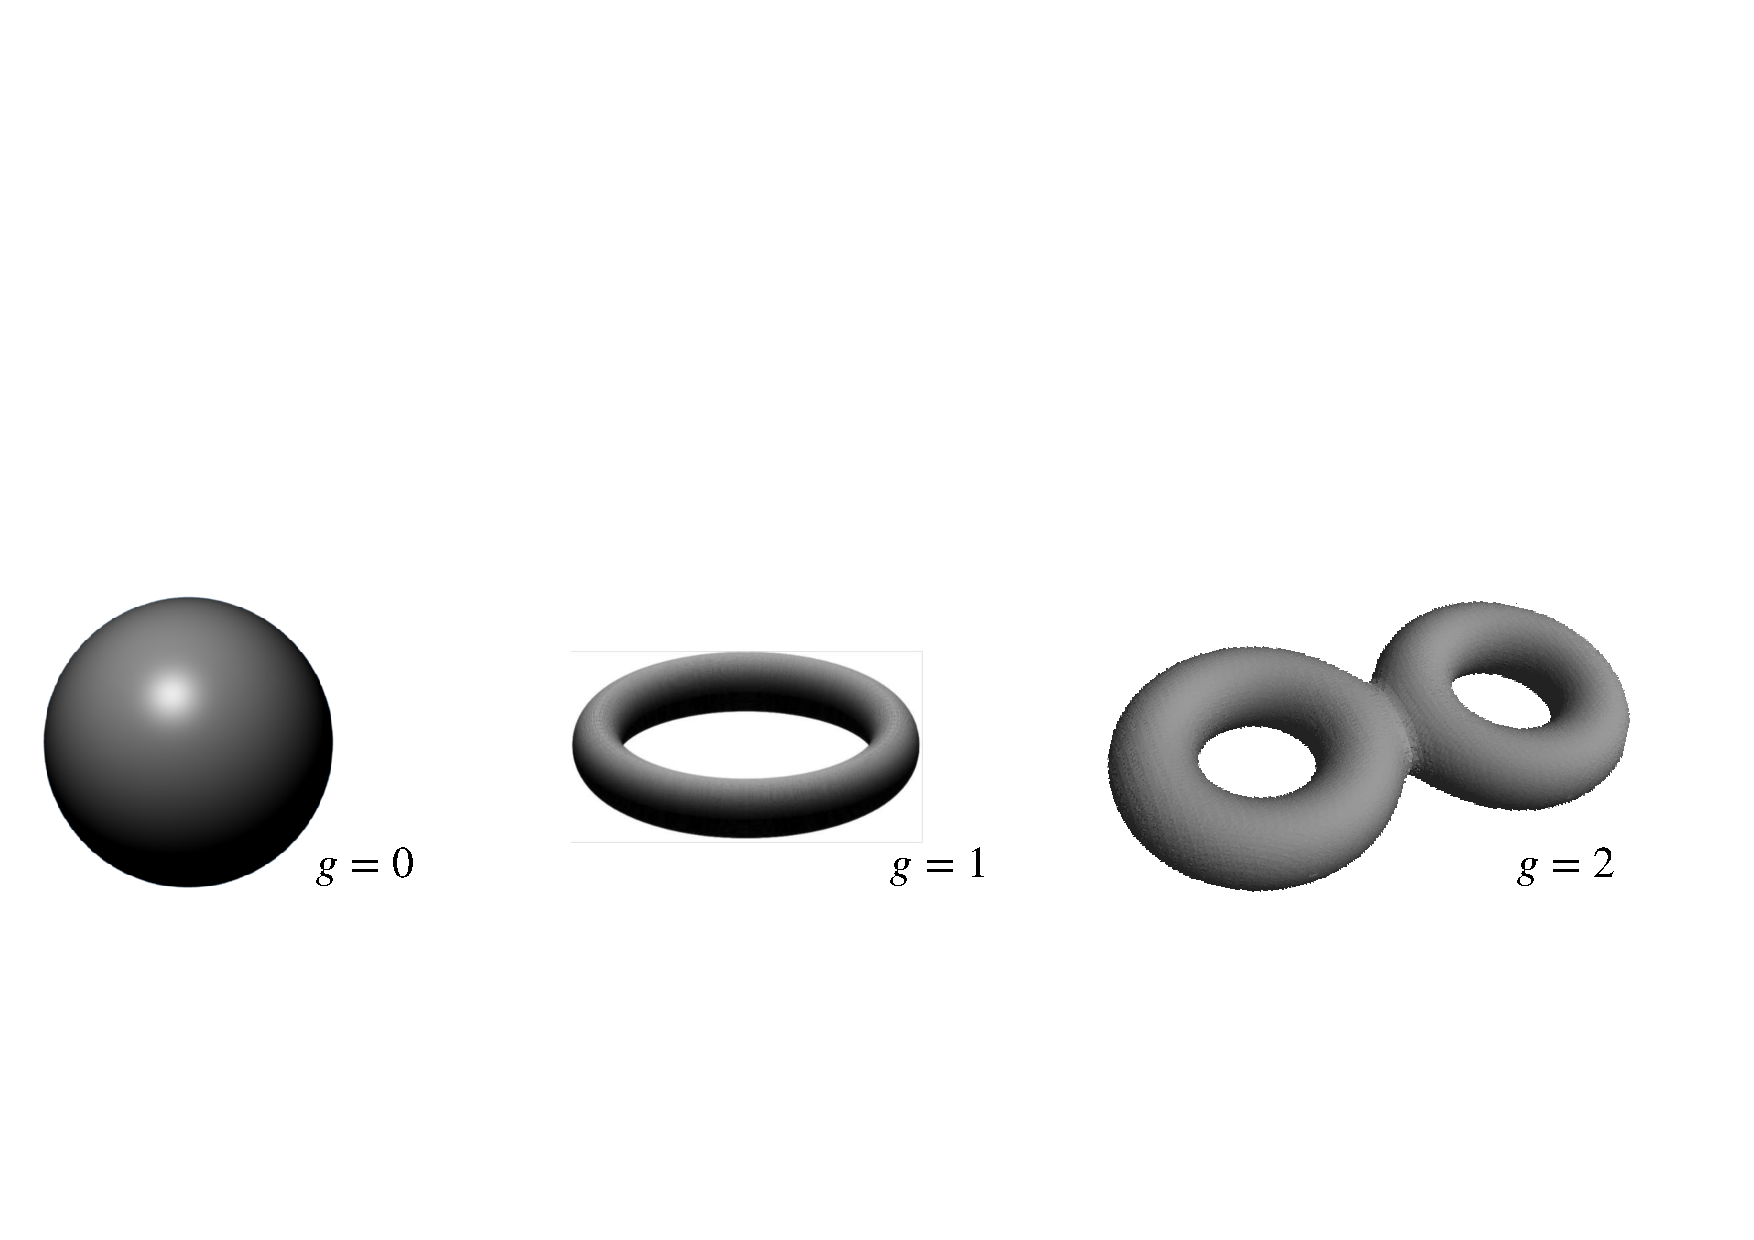
\includegraphics[width=6in]{\MemTB/Pics/genus}
\caption{
به ترتیب از چپ به راست یک کُره، چنبره، و دو چنبره متصل به هم را مشاهده می‌کند که به ترتیب شکلی با 
$0$
،
$1$
، و 
$2$
سوراخ/دسته که همچنین مقدار جینوس این سطوح را تعیین می‌کند.
}
\label{fig:genus012}
\end{center}
\end{figure}
برای مثال انرژی انحنای یک کُره به شعاع
$R$
را با استفاده از معادلات
\ref{eq:HelfrichBendingEnergy}
و
\ref{eq:HelfrichGaussianEnergy}
محاسبه می‌کنیم. با فرض اینکه بردار عمود بر سطح کره در جهت خارج کُره تعریف شده باشد، از انجایی که شعاع‌ کره در تمام نقاط سطح آن ثابت است خمش در سراسر سطح با یک مقدار
$C_1=C_2=1/R$
تعیین می‌شود. تنها فرض باقی مانده تعیین خمش ذاتی شکل است. در صورتی که فرض شود حالت تعادلی رویه‌ای که کُره را تشکیل داده سطح تخت باشد
$C_0=0$
انرژی آن
 \begin{equation}
 \begin{aligned}
E_{b}&=\frac{1}{2}\kappa\int R^2d\Omega (\frac{2}{R}-0)^2=8\pi\kappa\\
E_{G}&=\kappa_G\int R^2d\Omega \frac{1}{R^2}=4\pi\kappa_G=2\pi\kappa_G(2-2g)=2\pi\kappa_G(2-0) \\
E_{cu}&=8\pi\kappa+4\pi\kappa_G
\end{aligned}
\end{equation}
و در صورتی که خمش ذاتی آن
$C_0=1/R$
باشد انرژی انحنای آن
 \begin{equation}
 \begin{aligned}
E_{b}&=\frac{1}{2}\kappa\int R^2d\Omega (\frac{2}{R}-\frac{2}{R})^2=0\\
E_{G}&=2\pi\kappa_G(2-2g)=4\pi\kappa_G \\
E_{cu}&=4\pi\kappa_G
\end{aligned}
\end{equation}
است. توجه کنید که انرژی انحنای محاسبه شده تابع شعاع کُره نیست. به طور عمومی انرژی محاسبه شده با مدل خمش ذاتی از مقیاس شکل مستقل است. در نتیجه مدول خمشی
$\kappa$
نیز تابع مقیاس سیستم نخواهد بود. این مفهوم بسیار متفاوت از تعاریف رایج از مدول خمشی برای پلیمر‌هاست و باید توجه ویژه‌ای به این نکته بشود. از آنجایی که در مطالعه‌ی شکل غشا معمولا اختلاف انرژی بین اشکال اهمیت دارد و (به خصوص برای محاسبه‌ی نیرو) تا زمانی که غشا تغییر توپولوژیکی نداشته باشد، از محاسبه‌ی مقدار ثابت انرژی خمش گاووسی چشم پوشی می‌شود. 




































